\begin{figure}
	\centering
	\begin{tikzpicture}
		\node[anchor=south west, inner sep=0](image) at (0,0){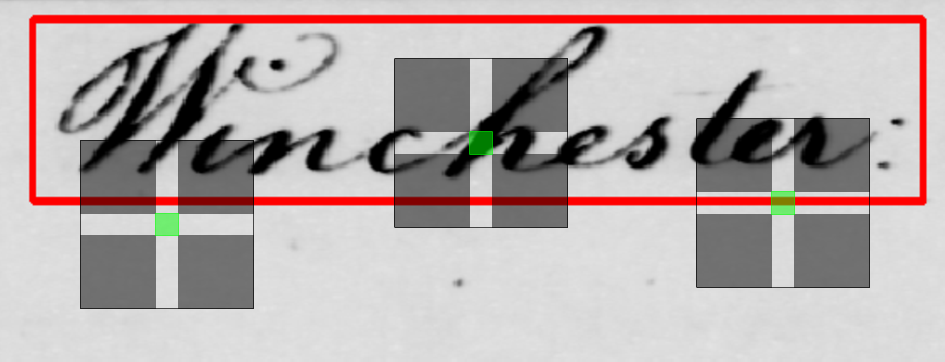
\includegraphics[width=.9\columnwidth]{images/lrc_crossmask_label_example.pdf}};
		\begin{scope}[x={(image.south east)},y={(image.north west)}]
	    %\tikzhelpergrid
		 \node[anchor=west] at (0.44, 0.31) {Inside};
		 \node[anchor=west] at (0.096, 0.09) {Outside};
		 \node[anchor=west] at (0.73, 0.14) {Intersects};
		\end{scope}
	\end{tikzpicture}
	\caption{Exemplary input to the LRC detector representing the three classes \emph{inside}, \emph{intersects}, and \emph{outside}. All parts marked with gray are ignored when processing the local regions with the CNN. Class membership is determined by the position of the crosses' intersection w.r.t. word bounding boxes.}
	\label{fig:lrc}
\end{figure}
